\documentclass{beamer}
\usetheme{colmex}
\renewcommand{\tablename}{Cuadro}

\presentador{Equipo 1}

% Barra inferior: navegación por secciones encima de la barra azul
\setbeamertemplate{navigation symbols}{}
\setbeamertemplate{footline}{%
  \leavevmode%
  \vbox{%
    \hbox{\insertnavigation{\paperwidth}}%
    \vskip2pt%
    \hbox{%
      \begin{beamercolorbox}[wd=\paperwidth,ht=2.25ex,dp=1ex]{footline}%
        \hspace*{2ex}\usebeamerfont{author in head/foot}\insertshortauthor
        \hfill\insertframenumber{} / \inserttotalframenumber\hspace*{2ex}%
      \end{beamercolorbox}}%
  }%
}
% Paquetes estandar utilizados en las diapositivas de identificacion.
% No cambian el tema colmex ni requieren archivos externos adicionales.
\usepackage{amsmath,amssymb}
\usepackage{booktabs}
\usepackage{array}
\usepackage{graphicx}
\usepackage{caption}
\usetikzlibrary{arrows.meta}

\title{Efectos de un choque de política monetaria en Colombia}
\subtitle{VAR estructural (SVAR)}
\author[Equipo 1]{Oscar Daniel Hernández Romero, Kevin Mejía Rodríguez y Rubén Perea Cervantes}
\date{Macroeconometría \textperiodcentered\ Otoño 2026}

% Portada de cada seccion, respetando el tema del proyecto original.
\AtBeginSection[]{%
  \begin{frame}[plain,noframenumbering]
    \vfill
    \begin{center}
      {\fontsize{26}{30}\selectfont\bfseries\color{azulraf}\insertsectionhead\par}
      \vspace{0.35cm}
      {\color{azulraf}\rule{0.35\textwidth}{1.2pt}\par}
    \end{center}
    \vfill
  \end{frame}
}

% Nota discreta para referencias al pie de las diapositivas.
\newcommand{\refslide}[1]{\par\vspace{0.12cm}{\tiny\color{gray}\emph{#1}}}

\begin{document}

\portada

% =============================================================================
\section{Introducción}

\begin{frame}{Pregunta y estrategia}
  \framesubtitle{¿Qué efectos tiene un alza de la tasa de política en Colombia?}
  \begin{itemize}
    \item Respuesta de la \textbf{actividad}, la \textbf{inflación}, sus
    \textbf{expectativas} y el \textbf{tipo de cambio real} a un choque de política monetaria.
    \item Colombia: economía pequeña y abierta, tipo de cambio flexible y metas de
    inflación desde 1999 (meta de 3\,\% desde 2010).
    \item Características similares a las de México.
  \end{itemize}
  \vfill
  \begin{block}{Estrategia}
    SVAR de cinco variables con datos mensuales, 2010--2026.\\
    Identificación con restricciones de \alert{corto y largo plazo}
    (combinación 1), siguiendo a Bj{\o}rnland (2009).
  \end{block}
\end{frame}

% =============================================================================
\section{Datos}

\begin{frame}{Datos}
  \framesubtitle{Mensuales, 2010m1--2026m7 ($T=199$), fuentes oficiales}
  \begin{columns}[T]
    \begin{column}{0.54\textwidth}
      \begin{block}{Endógenas}
        \small
        \begin{itemize}
          \item ISE (actividad) --- DANE
          \item Inflación (IPC) --- DANE
          \item Expectativas de inflación a 12 meses --- BanRep
          \item TPM (instrumento) --- BanRep
          \item ITCR (canal cambiario) --- BanRep
        \end{itemize}
      \end{block}
    \end{column}
    \begin{column}{0.44\textwidth}
      \begin{block}{Exógenas, en $t$ y $t-1$}
        \small
        \begin{itemize}
          \item Precio del Brent
          \item Tasa de la Fed
        \end{itemize}
        Colombia no influye en ellas, pero ellas sí en Colombia.
      \end{block}
    \end{column}
  \end{columns}
  \vfill
  \begin{alertblock}{¿Por qué mensual?}
    Permite estudiar la transmisión de corto plazo, aunque exige justificar
    cuidadosamente las exclusiones dentro del mes.
  \end{alertblock}
\end{frame}

\begin{frame}{Las series}
  \framesubtitle{Variables endógenas, tal como entran al VAR}
  \begin{center}
    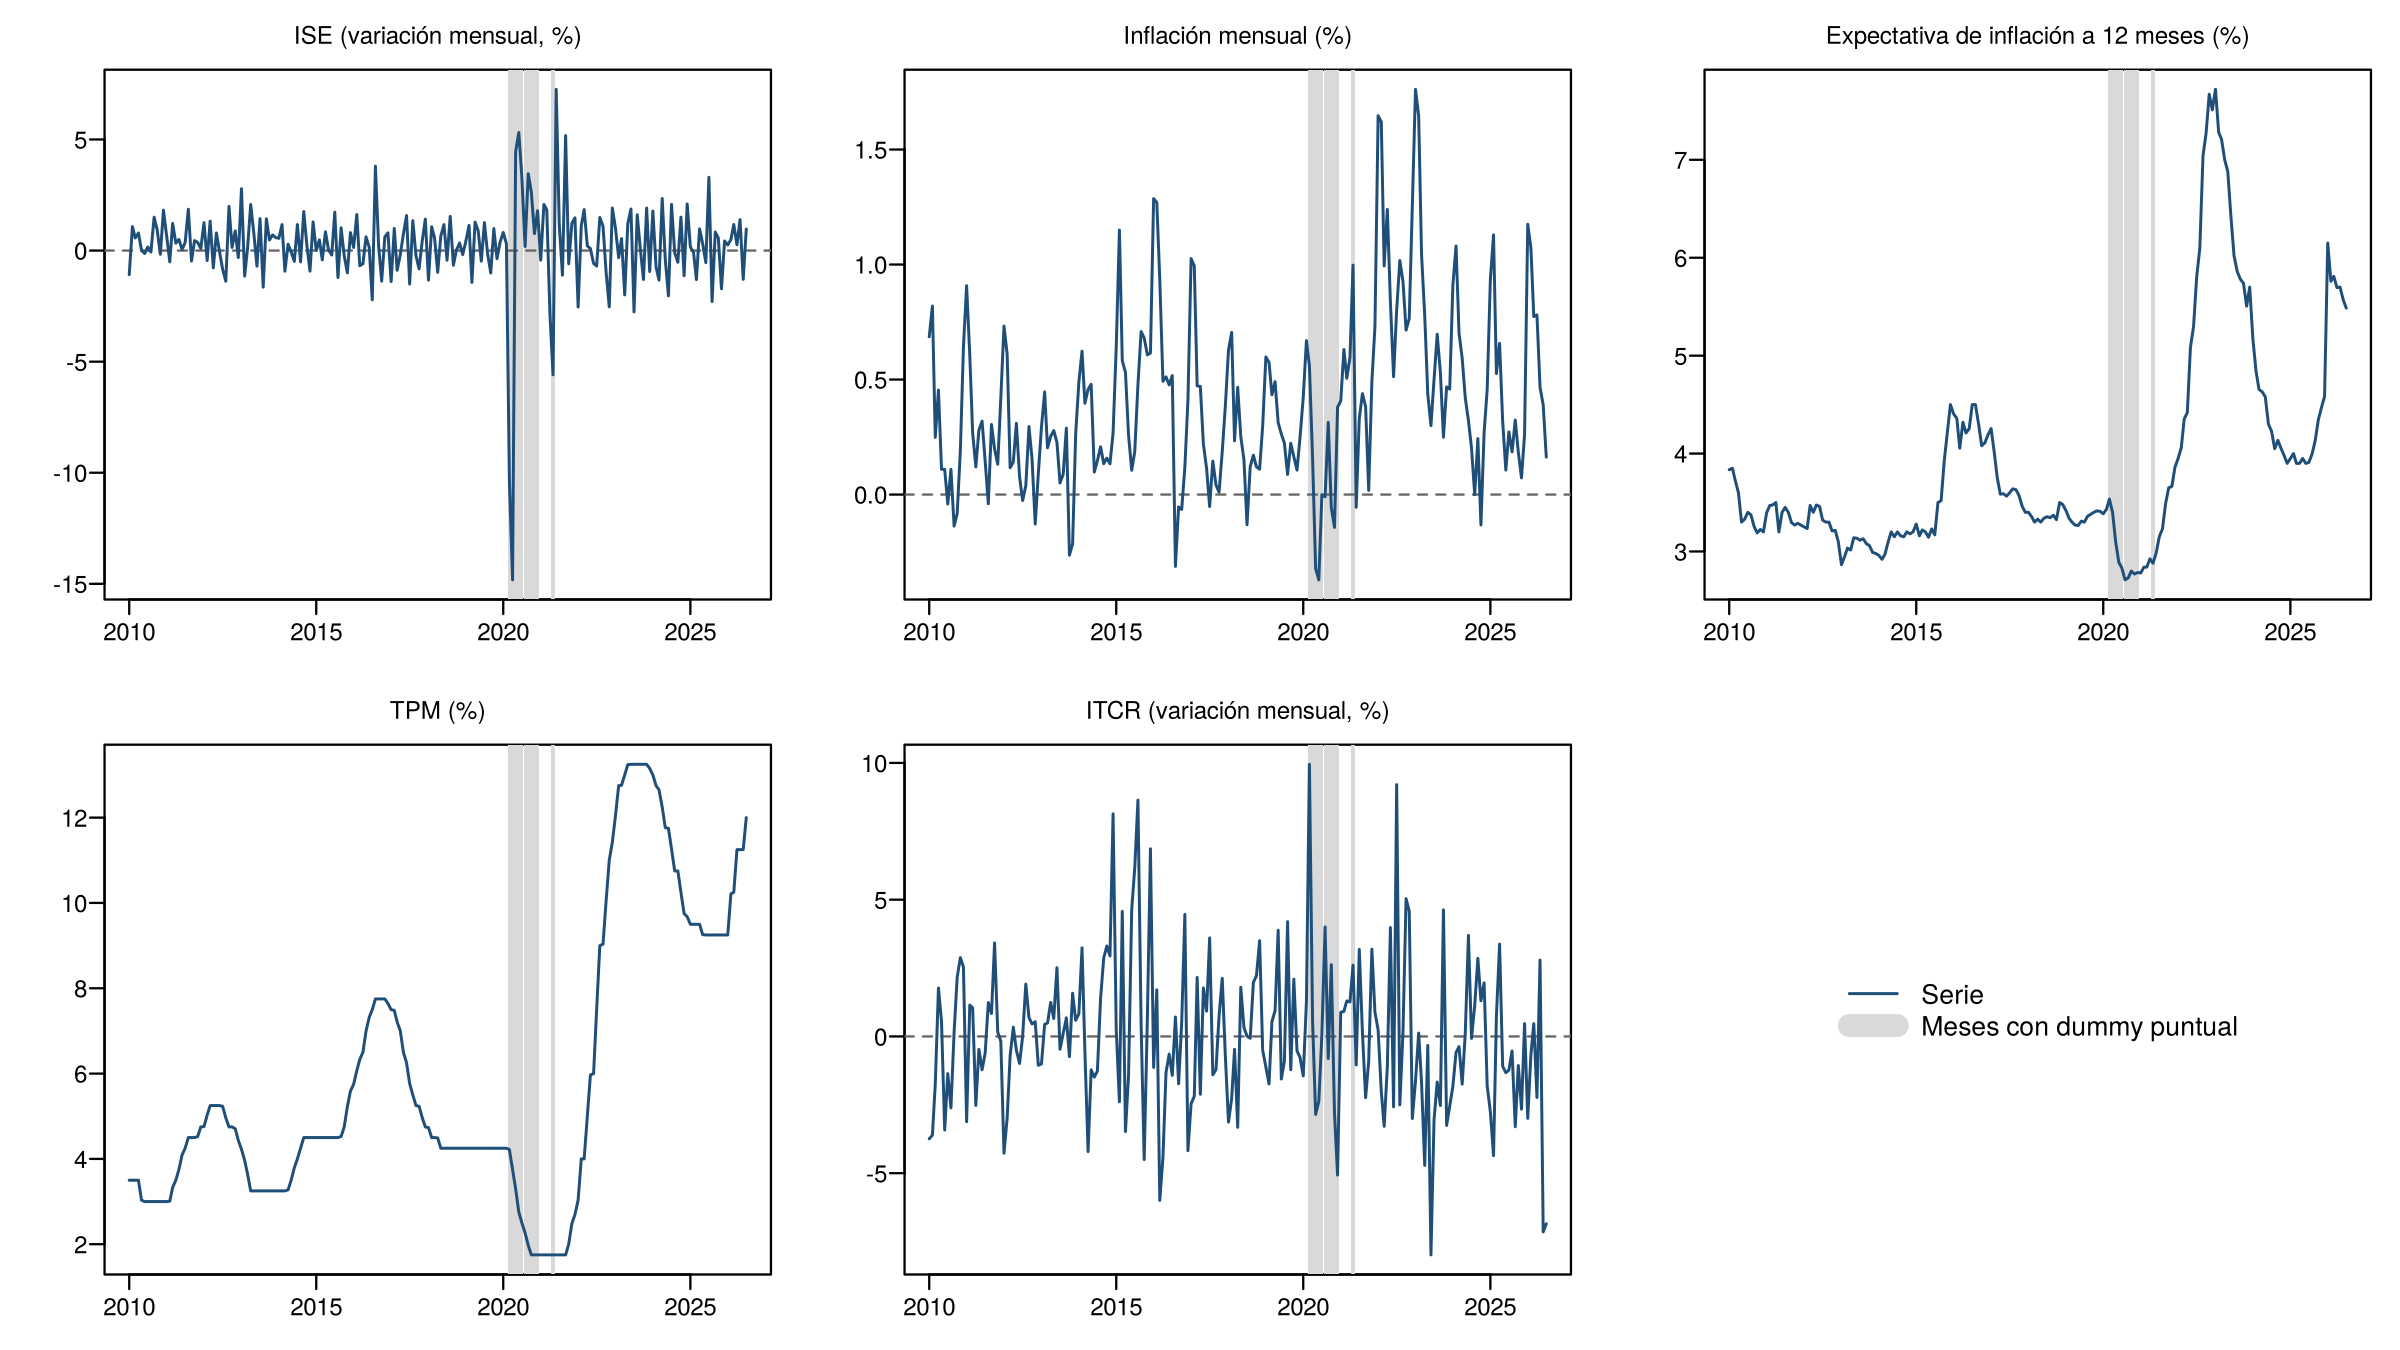
\includegraphics[width=\textwidth]{img/fig_series_presentacion.png}
  \end{center}
  \vspace{-0.4cm}
  {\tiny Área gris: \textit{dummies} puntuales (mar--dic 2020, pandemia; may 2021, paro nacional).}
\end{frame}

\begin{frame}{Transformaciones}
  \framesubtitle{Guiadas por las pruebas ADF y KPSS}
  \begin{center}
  \scriptsize
  \renewcommand{\arraystretch}{1.3}
  \begin{tabular}{lll}
    \toprule
    \textbf{Variable} & \textbf{Entra al VAR como} & \textbf{Por qué} \\
    \midrule
    ISE & Variación mensual del log & Raíz unitaria en nivel \\
    ITCR & Variación mensual del log & Raíz unitaria; restricción de largo plazo \\
    Inflación & Variación mensual del log del IPC & Estacionaria sin el patrón estacional \\
    Expectativas & Nivel & Interpretación del anclaje \\
    TPM & Nivel (promedio mensual) & El choque se lee como cambio en la tasa \\
    \bottomrule
  \end{tabular}
  \end{center}
  \vfill
  \begin{block}{ITCR en diferencias}
    La restricción de largo plazo exige que el \alert{nivel} del tipo de cambio real
    regrese a su trayectoria de referencia: la suma de sus respuestas mensuales es cero.
  \end{block}
\end{frame}

\begin{frame}{Estacionalidad del IPC}
  \framesubtitle{¿Inflación mensual con \textit{dummies} o inflación anual?}
  \begin{columns}[c]
    \begin{column}{0.56\textwidth}
      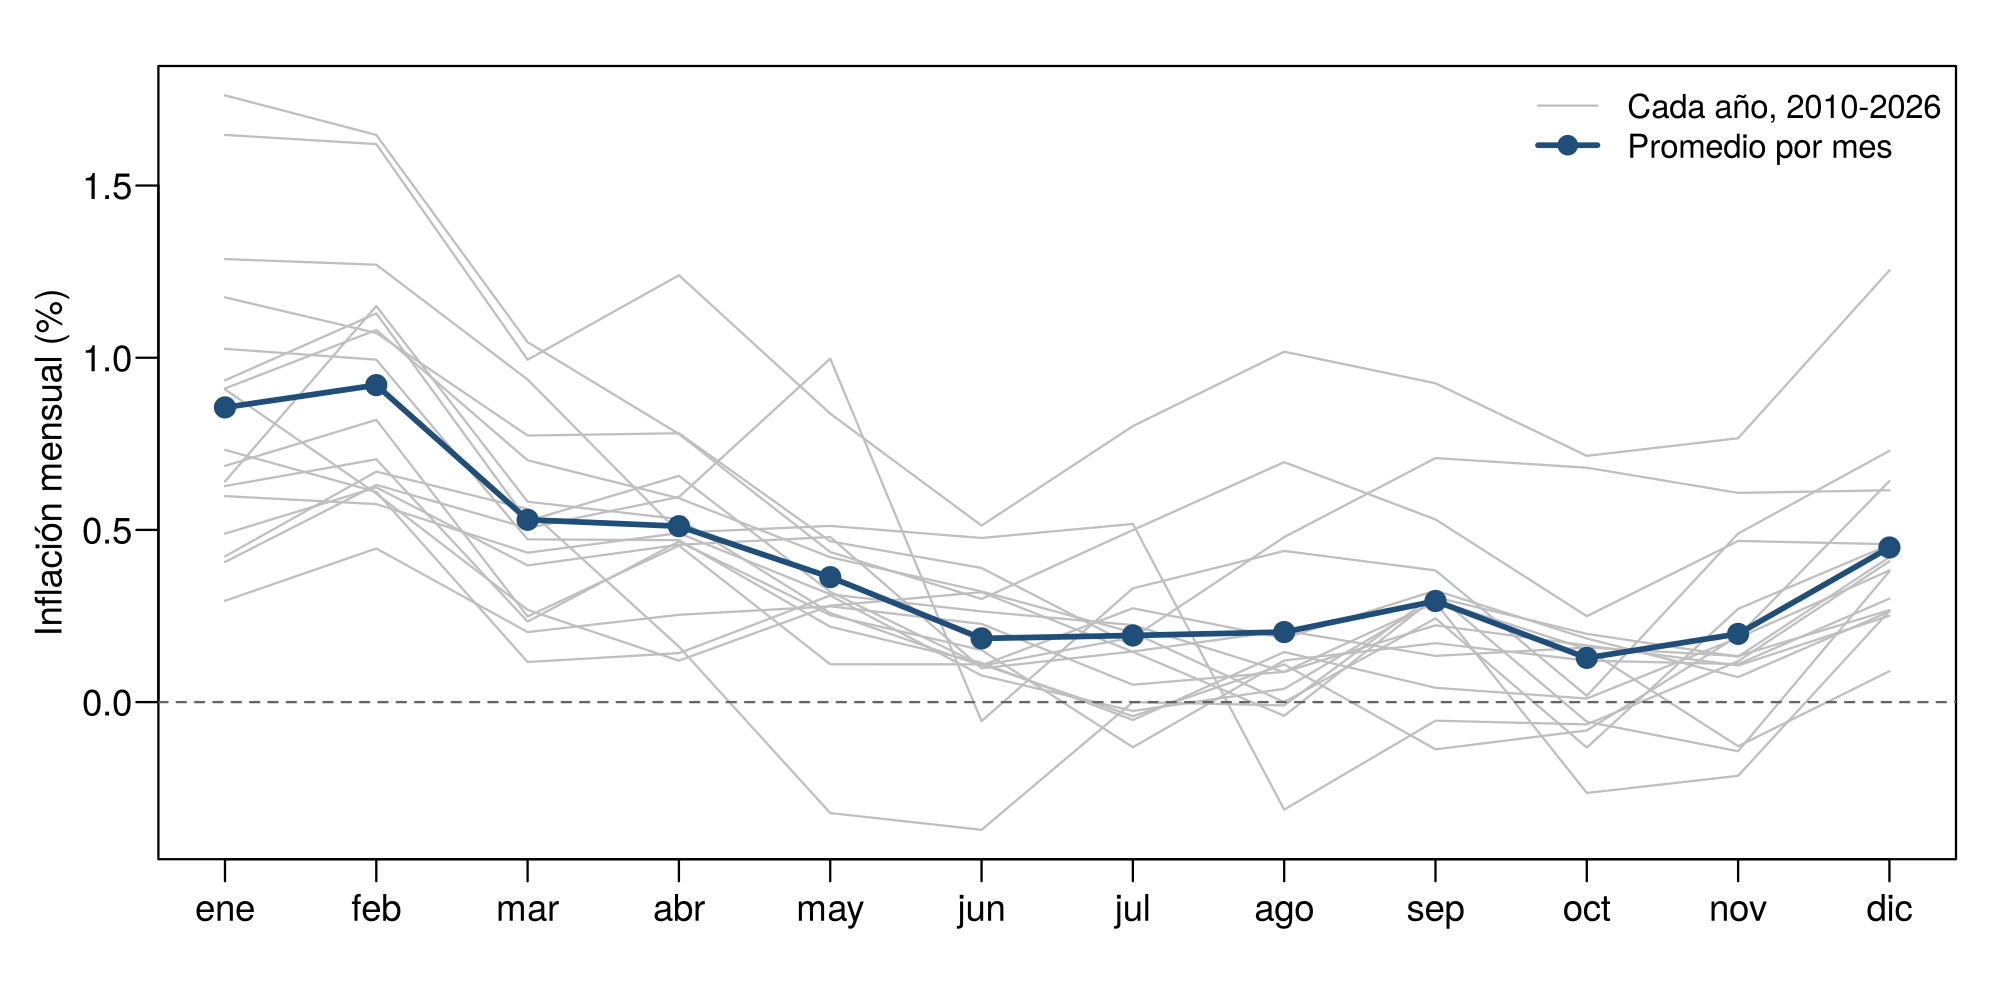
\includegraphics[width=\textwidth]{img/fig_estacionalidad.png}
    \end{column}
    \begin{column}{0.42\textwidth}
      \small
      \begin{itemize}
        \item El IPC no está desestacionalizado.
        \item \textbf{OCSB}: rechaza raíz unitaria estacional.
        \item \textbf{Canova--Hansen}: no rechaza estacionalidad estable.
      \end{itemize}
    \end{column}
  \end{columns}
  \vfill
  \begin{alertblock}{Decisión}
    El patrón se repite cada año: inflación \alert{mensual} con 11 \textit{dummies}
    estacionales. Con inflación anual, el VAR(6) no es estable.
  \end{alertblock}
\end{frame}

% =============================================================================

\section{Identificación}

\begin{frame}{Estrategia: corto y largo plazo}
 \framesubtitle{Adaptación del enfoque de Bj{\o}rnland (2009) a Colombia}
 \begin{columns}[T]
  \begin{column}{0.49\textwidth}
   \begin{block}{Corto plazo}
    \small
    \textbf{Nueve restricciones contemporáneas} entre actividad económica,
    inflación y expectativas de inflación.\\
   \end{block}
  \end{column}
  \begin{column}{0.49\textwidth}
   \begin{block}{Largo plazo}
    \small
    \textbf{Una restricción de largo plazo:} el choque de política monetaria no desplaza
    permanentemente el \emph{nivel} del tipo de cambio real.\\
   \end{block}
  \end{column}
 \end{columns}
 \vfill
 \begin{alertblock}{¿Qué identificamos?}
  \small Una perturbación que eleva la tasa de política monetaria al impacto y satisface las diez
  restricciones. Sin embargo, su interpretación \emph{causal} exige supuestos adicionales.
 \end{alertblock}
\end{frame}

\begin{frame}{Restricciones necesarias}
 \framesubtitle{Identificación por orden en un sistema de cinco variables}
 \begin{columns}[c]
  \begin{column}{0.31\textwidth}
   \begin{block}{Incógnitas}
    \centering\LARGE $25$\\[0.3em]
    \scriptsize coeficientes en $H$
   \end{block}
  \end{column}
  \begin{column}{0.31\textwidth}
   \begin{block}{Información}
    \centering\LARGE $15$\\[0.3em]
    \scriptsize momentos en $\Sigma_u$
   \end{block}
  \end{column}
  \begin{column}{0.31\textwidth}
   \begin{alertblock}{Faltan}
    \centering\LARGE $10$\\[0.3em]
    \scriptsize igualdades independientes
   \end{alertblock}
  \end{column}
 \end{columns}
 \vspace{0.4cm}
 \begin{equation*}
 K^2-\frac{K(K+1)}{2}=\frac{K(K-1)}{2}=10,\qquad K=5.
 \end{equation*}
 \vfill
 \begin{block}{Cómo las completamos}
   \centering\small \textbf{Nueve ceros de impacto} $+$ \textbf{una neutralidad de largo plazo}.
 \end{block}
\end{frame}

\begin{frame}{Matriz de impacto}
 \begin{equation*}
 H=\begin{pmatrix}
 h_{11}&0&0&0&0\\
 h_{21}&h_{22}&0&0&0\\
 h_{31}&h_{32}&h_{33}&0&0\\
 h_{41}&h_{42}&h_{43}&\alert{h_{44}}&\alert{h_{45}}\\
 h_{51}&h_{52}&h_{53}&\alert{h_{54}}&h_{55}
 \end{pmatrix}, \qquad \alert{h_{44}>0}.
 \end{equation*}
 \begin{columns}[T]
  \begin{column}{0.49\textwidth}
   \begin{block}{Ceros impuestos}
   \scriptsize
   $h_{12}=h_{13}=h_{14}=h_{15}=0$\\
   $h_{23}=h_{24}=h_{25}=0$\\
   $h_{34}=h_{35}=0$
   \end{block}
  \end{column}
  \begin{column}{0.49\textwidth}
   \begin{block}{Interacción permitida}
    \scriptsize
    $h_{45}$: TPM ante shock cambiario.\\
    $h_{54}$: ITCR ante shock monetario.\\
    \alert{No se exige apreciación al impacto.}
   \end{block}
  \end{column}
 \end{columns}
\end{frame}

\begin{frame}{Actividad económica}
 \framesubtitle{Cuatro restricciones contemporáneas}
 \scriptsize
 \renewcommand{\arraystretch}{1.32}
 \begin{tabular}{@{}p{0.105\linewidth}p{0.41\linewidth}p{0.41\linewidth}@{}}
 \toprule
 \textbf{Cero} & \textbf{Motivación económica} & \textbf{Límite del supuesto}\\
 \midrule
 $h_{12}=0$ & Producción y gasto no se ajustan inmediatamente ante noticias de precios. & Shocks de oferta pueden mover producción y precios juntos.\\
 $h_{13}=0$ & La realización de planes de gasto e inversión toma tiempo. & Las noticias sobre inflación pueden alterar decisiones actuales.\\
 $h_{14}=0$ & El canal monetario hacia demanda y producción opera con rezagos. & Crédito y decisiones financieras pueden ajustarse en el mes.\\
 $h_{15}=0$ & El canal comercial y de balances del tipo de cambio requiere ajuste. & Importadores, exportadores y deudores en divisas pueden reaccionar rápidamente.\\
 \bottomrule
 \end{tabular}
 \vfill
  \small Se imponen cuatro \emph{ceros mensuales exactos}; la teoría de transmisión gradual
 los motiva, pero no los demuestra de forma independiente.
\end{frame}

\begin{frame}{Inflación mensual}
 \framesubtitle{Tres restricciones al impacto}
 \scriptsize
 \renewcommand{\arraystretch}{1.30}
 \begin{tabular}{@{}p{0.105\linewidth}p{0.39\linewidth}p{0.435\linewidth}@{}}
 \toprule
 \textbf{Cero} & \textbf{Motivación económica} & \textbf{Alcance y evidencia colombiana}\\
 \midrule
 $h_{23}=0$ & Los precios no incorporan inmediatamente toda innovación de expectativas. & Sánchez-Jabba y Villabón-Hinestroza (2024) encuentran un traspaso importante de expectativas a inflación; no prueban un cero inmediato.\\
 $h_{24}=0$ & Los efectos de la TPM sobre demanda y precios se distribuyen en el tiempo. & González-Téllez y Laborde-Vera (2026) documentan efectos desinflacionarios dinámicos; no identifican una ausencia exacta en el mes.\\
 $h_{25}=0$ & El movimiento cambiario pasa por precios importados, costos y márgenes antes del IPC. & Rowland (2004) y Larrahondo et al. (2025) encuentran traspaso incompleto y pequeño en IPC, pero no necesariamente nulo.\\
 \bottomrule
 \end{tabular}
 \vfill
\end{frame}

\begin{frame}{Expectativas de inflación}
 \framesubtitle{Dos restricciones contemporáneas por efectos de calendario}
 \begin{block}{Hecho institucional}
  \small La Encuesta Mensual de Expectativas se levanta habitualmente entre los
  \textbf{días 6 y 14}, mientras que TPM e ITCR son medidas mensuales.
 \end{block}
 \vspace{0.2cm}
 \begin{columns}[T]
  \begin{column}{0.48\textwidth}
   \begin{block}{$h_{34}=0$: TPM}
    \small Una sorpresa monetaria posterior al levantamiento no puede modificar
    la encuesta ya respondida.
   \end{block}
  \end{column}
  \begin{column}{0.48\textwidth}
   \begin{block}{$h_{35}=0$: ITCR}
    \small Una perturbación cambiaria posterior al levantamiento tampoco puede
    modificar respuestas anteriores.
   \end{block}
  \end{column}
 \end{columns}
 \vfill
 \begin{alertblock}{}
  \small Las decisiones pueden anticiparse y el ITCR contiene movimientos
  \alert{anteriores} a la encuesta. El calendario no garantiza ceros exactos.
 \end{alertblock}
\end{frame}

\begin{frame}{Qué dejamos libre}
 \begin{columns}[c]
  \begin{column}{0.47\textwidth}
   \begin{block}{Shock monetario $\varepsilon_{4t}$}
    \centering
    \large $h_{44}>0$\\[0.45em]
    \normalsize $h_{54}$ libre\\[0.45em]
    \small El ITCR puede apreciarse o depreciarse en el mes de la contracción.
   \end{block}
  \end{column}
  \begin{column}{0.47\textwidth}
   \begin{block}{Shock cambiario $\varepsilon_{5t}$}
    \centering
    \large $h_{45}$ libre\\[0.45em]
    \normalsize $h_{55}$ libre\\[0.45em]
    \small El Banco puede modificar la TPM ante perturbaciones cambiarias.
   \end{block}
  \end{column}
 \end{columns}
 \vfill
 \begin{alertblock}{Ventaja y limitaciones}
  \small Se permite la interacción contemporánea. Sin embargo, eso no garantiza
  separar completamente shocks monetarios de primas de riesgo o intervenciones cambiarias.
 \end{alertblock}
\end{frame}

\begin{frame}{Neutralidad de largo plazo del ITCR}
 \framesubtitle{La décima restricción completa la identificación por orden}
 \small
 \begin{equation*}
 A(1)=I_5-\sum_{j=1}^{6}A_j,\qquad
 \Theta_h=\Psi_hH,\qquad
 \sum_{h=0}^{\infty}\Theta_h=A(1)^{-1}H.
 \end{equation*}
 \vspace{0.1cm}
 \begin{alertblock}{Condición}
 \centering
 \Large $\displaystyle \boxed{e_5' A(1)^{-1} H e_4=0.}$
 \end{alertblock}
 \begin{itemize}
  \item La quinta variable es el \textbf{crecimiento mensual del ITCR}.
  \item Su respuesta \emph{acumulada} aproxima la variación del \textbf{nivel} real.
  \item La suma de las respuestas mensuales al shock monetario es \textbf{cero a horizonte infinito}.
  \item Que el ITCR acumulado regrese a cero \textbf{no es una prueba empírica}
  de neutralidad: es una condición utilizada para identificar el shock.
 \end{itemize}
\end{frame}

\begin{frame}{Normalización del shock a 25 puntos base}
 \small
 \begin{equation*}
 \underbrace{h_{44}}_{\text{impacto, 1 desv. est.}}=0.161\ \text{pp},
 \qquad \underbrace{\frac{0.25}{h_{44}}}_{\text{factor de escala}}
 \simeq 1.55.
 \end{equation*}
 \begin{block}{Respuesta monetaria normalizada}
 \centering
 \large $\displaystyle IRF_j(h;25\,pb)=\frac{0.25}{0.161}\,e_j'\Psi_h\widehat H e_4.$
 \end{block}
 \begin{itemize}
  \item La normalización \textbf{no agrega una restricción identificadora}.
  \item El signo $h_{44}>0$ define una contracción monetaria.
  \item Para ISE e ITCR se muestran \textbf{respuestas acumuladas}.
 \end{itemize}
\end{frame}

\begin{frame}{Identificación estructural y límites causales}
 \footnotesize
 \begin{itemize}
  \item \textbf{1.} \textbf{Temporalidad mensual:} encuesta (días 6--14) frente a promedios de TPM e ITCR.
  \item \textbf{2.} \textbf{Información de la autoridad monetaria:} el Banco de la República puede reaccionar a previsiones no observadas por el VAR.
  \item \textbf{3.} \textbf{Otros shocks:} primas de riesgo, intervenciones cambiarias y perturbaciones financieras.
  \item \textbf{4.} \textbf{Neutralidad impuesta:} las fricciones reales y financieras pueden alterar efectos de largo plazo.
  \item \textbf{5.} \textbf{Controles externos incompletos:} Brent y Fed no agotan los determinantes externos.
 \end{itemize}
 \vspace{0.06cm}
 \begin{alertblock}{Alcance de la identificación}
 \footnotesize Efectos dinámicos \textbf{condicionados} a las restricciones; la interpretación como shock
 monetario \emph{puramente exógeno} exige supuestos adicionales.
 \end{alertblock}
\end{frame}

% =============================================================================
\section{Estimación}

\begin{frame}{Estimación}
  \framesubtitle{VAR en forma reducida por MCO, ecuación por ecuación}
  \begin{columns}[T]
    \begin{column}{0.48\textwidth}
      \begin{block}{Método}
        \small
        Mismos regresores en todas las ecuaciones: MCO por ecuación equivale a
        estimar el sistema completo.\\[0.2em]
        57 regresores por ecuación.
      \end{block}
    \end{column}
    \begin{column}{0.48\textwidth}
      \scriptsize
      \begin{center}
      \textbf{Selección de rezagos}\\[0.25em]
      \begin{tabular}{lc}
        \toprule
        Criterio & Rezagos \\
        \midrule
        Akaike & 5 \\
        Hannan--Quinn & 4 \\
        Schwarz & 1 \\
        \midrule
        \textbf{Elegido} & \alert{\textbf{6}} \\
        \bottomrule
      \end{tabular}
      \end{center}
    \end{column}
  \end{columns}
  \vfill
  \begin{block}{¿Por qué seis?}
    El mayor sugerido por los criterios más uno: omitir rezagos puede distorsionar las
    respuestas de largo plazo (Kilian y Lütkepohl, 2017). Robustez con 4 y 8.
  \end{block}
\end{frame}

\begin{frame}{Diagnósticos}
  \framesubtitle{VAR con seis rezagos}
  \begin{center}
  \scriptsize
  \renewcommand{\arraystretch}{1.3}
  \begin{tabular}{@{}p{0.34\textwidth}p{0.26\textwidth}p{0.30\textwidth}@{}}
    \toprule
    \textbf{Prueba} & \textbf{Resultado} & \textbf{Lectura} \\
    \midrule
    Raíz más grande & 0.949 & Estable \\
    Portmanteau, 24 meses & $p=0.131$ & No rechaza $H_0$ \\
    LM, orden 1 & $p=0.242$ & No rechaza \\
    LM, orden 12 & $p=0.004$ & \alert{Rechaza} \\
    Ljung-Box por ecuación & Sin rechazos al 5\% & No rechaza $H_0$ \\
    ARCH-LM & Rechaza en ISE y TPM & Varianza no constante \\
    Jarque-Bera & Rechaza en ISE, inflación y expectativas & No normalidad \\
    \bottomrule
  \end{tabular}
  \end{center}
  \vfill
  \begin{alertblock}{Implicación para la inferencia}
    La estabilidad es favorable, pero los diagnósticos no son uniformes:
    se detecta autocorrelación con LM a 12 rezagos y heterocedasticidad.
  \end{alertblock}
\end{frame}

\begin{frame}{Estimación del SVAR}
  \framesubtitle{De $\hat\Sigma_u$ a la matriz de impacto $\hat H$}
  \small
  \begin{enumerate}[label=\arabic*.]
    \item \textbf{Cholesky:} $\hat\Sigma_u = PP'$, con $P$ triangular inferior.
    Ya cumple los \alert{nueve ceros} de impacto.
    \item \textbf{Rotación:} $\hat H = P\,Q(\theta)$, donde $Q(\theta)$ solo gira las columnas
    de TPM e ITCR. Conserva $\hat H\hat H'=\hat\Sigma_u$ y los nueve ceros.
    \item \textbf{Ángulo:} se elige $\theta$ para cumplir la neutralidad de largo plazo.
    Con $L=\hat A(1)^{-1}P$,
    \[
      \tan\theta = -\,\frac{L_{54}}{L_{55}}
      \quad\Longrightarrow\quad \hat\theta = 5.9^\circ .
    \]
  \end{enumerate}
  \vfill
  \begin{block}{Solución única y sin optimización}
    Diez restricciones para diez parámetros libres: el sistema está exactamente
    identificado y $\hat H$ tiene solución cerrada.
  \end{block}
\end{frame}

\begin{frame}{Matriz de impacto estimada}
  \framesubtitle{Choque de una desviación estándar}
  \begin{center}
  \scriptsize
  \renewcommand{\arraystretch}{1.25}
  \setlength{\tabcolsep}{5pt}
  \begin{tabular}{lrrrrr}
    \toprule
    & \multicolumn{5}{c}{\textbf{Choque}} \\
    \cmidrule(l){2-6}
    \textbf{Variable} & ISE & Inflación & Expect. & \textbf{TPM} & ITCR \\
    \midrule
    ISE          & $1.032$  & $0$      & $0$     & $\mathbf{0}$      & $0$ \\
    Inflación    & $-0.024$ & $0.171$  & $0$     & $\mathbf{0}$      & $0$ \\
    Expectativas & $-0.024$ & $0.045$  & $0.176$ & $\mathbf{0}$      & $0$ \\
    TPM          & $-0.004$ & $0.053$  & $0.002$ & $\mathbf{0.161}$  & $-0.017$ \\
    ITCR         & $-0.187$ & $-0.129$ & $0.035$ & $\mathbf{-0.040}$ & $2.289$ \\
    \midrule
    \multicolumn{4}{l}{Efecto de largo plazo sobre el nivel del ITCR} & $\mathbf{0}$ & \\
    \bottomrule
  \end{tabular}
  \end{center}
  \vfill
  \begin{columns}[T]
    \begin{column}{0.48\textwidth}
      \begin{block}{Choque monetario}
        \scriptsize Sube la TPM 16 pb; el ITCR se aprecia levemente en el mes
        ($-0.04\,\%$), sin que se haya impuesto.
      \end{block}
    \end{column}
    \begin{column}{0.48\textwidth}
      \begin{block}{Ángulo pequeño}
        \scriptsize El choque está cerca del recursivo: la TPM casi no responde
        en el mes a un choque cambiario ($\hat h_{45}=-0.017$).
      \end{block}
    \end{column}
  \end{columns}
  \vspace{0.15cm}
\end{frame}

% =============================================================================
%  INFERENCIA, RESULTADOS Y CONCLUSIONES (Oscar)
%  Figuras: las mismas del Anexo D (img/irf_P1_*.png, img/irf_P9_vs_P1_25pb.png).
% =============================================================================
\section{Inferencia}

\begin{frame}{Método de inferencia}
  \framesubtitle{Bootstrap por bloques}
  \begin{itemize}
    \item Se usa \textbf{bootstrap por bloques}, ya que nuestra serie presenta
    \textbf{heterocedasticidad condicional}, y este es el método más recomendado para
    estos casos (Kilian y Lütkepohl, 2017).
  \end{itemize}
  \vfill
  \begin{columns}[T]
    \begin{column}{0.31\textwidth}
      \begin{block}{Réplicas}
        \centering\LARGE 2,000\\[0.3em]
        \scriptsize con el mismo VAR
      \end{block}
    \end{column}
    \begin{column}{0.31\textwidth}
      \begin{block}{Bloques}
        \centering\LARGE 12\\[0.3em]
        \scriptsize meses seguidos
      \end{block}
    \end{column}
    \begin{column}{0.31\textwidth}
      \begin{block}{Bandas}
        \centering\LARGE 68\,\%\\[0.3em]
        \scriptsize percentiles 16 y 84
      \end{block}
    \end{column}
  \end{columns}
  \vfill
  \refslide{Brüggemann, Jentsch y Trenkler (2016); Kilian y Lütkepohl (2017), sección 12.2.5.}
\end{frame}

\begin{frame}{Método resumido}
  \framesubtitle{Bootstrap por bloques, paso a paso}
  \vfill
  \centering
  \begin{tikzpicture}[
      paso/.style={draw=azulraf, fill=fondo, rounded corners=3pt, line width=0.6pt, align=center,
                   font=\scriptsize, text=destacado, minimum height=1cm, text width=1.9cm},
      flecha/.style={-{Stealth[length=2.2mm]}, line width=0.8pt, draw=azulraf}]
    \node[paso] (datos) at (0, 0)       {Datos};
    \node[paso] (var)   at (3.2, 0)     {VAR(6)};
    \node[paso] (res)   at (6.2, 0)     {Residuos};
    \node[paso] (blo)   at (9.2, 0)     {17 bloques\\de 12 meses};
    \node[paso] (serie) at (9.2, -1.7)  {Serie artificial};
    \node[paso] (varid) at (9.2, -3.4)  {VAR con la misma identificación};
    \node[paso] (resp)  at (5.7, -3.4)  {Respuestas\\(2,000 réplicas)};
    \node[paso, text width=2.5cm, line width=1.2pt] (band) at (1.9, -3.4)
         {Se ordenan y se toman los percentiles 16 y 84};
    \draw[flecha] (datos) -- node[above, font=\tiny, text=normal] {estimación} (var);
    \draw[flecha] (var) -- (res);
    \draw[flecha] (res) -- (blo);
    \draw[flecha] (blo) -- (serie);
    \draw[flecha] (serie) -- (varid);
    \draw[flecha] (varid) -- (resp);
    \draw[flecha] (resp) -- (band);
  \end{tikzpicture}
  \vfill
\end{frame}

% =============================================================================
\section{Resultados}

\begin{frame}{Resultados}
  \framesubtitle{Respuestas a un alza de 25 pb en la TPM: bootstrap por bloques}
  \begin{center}
    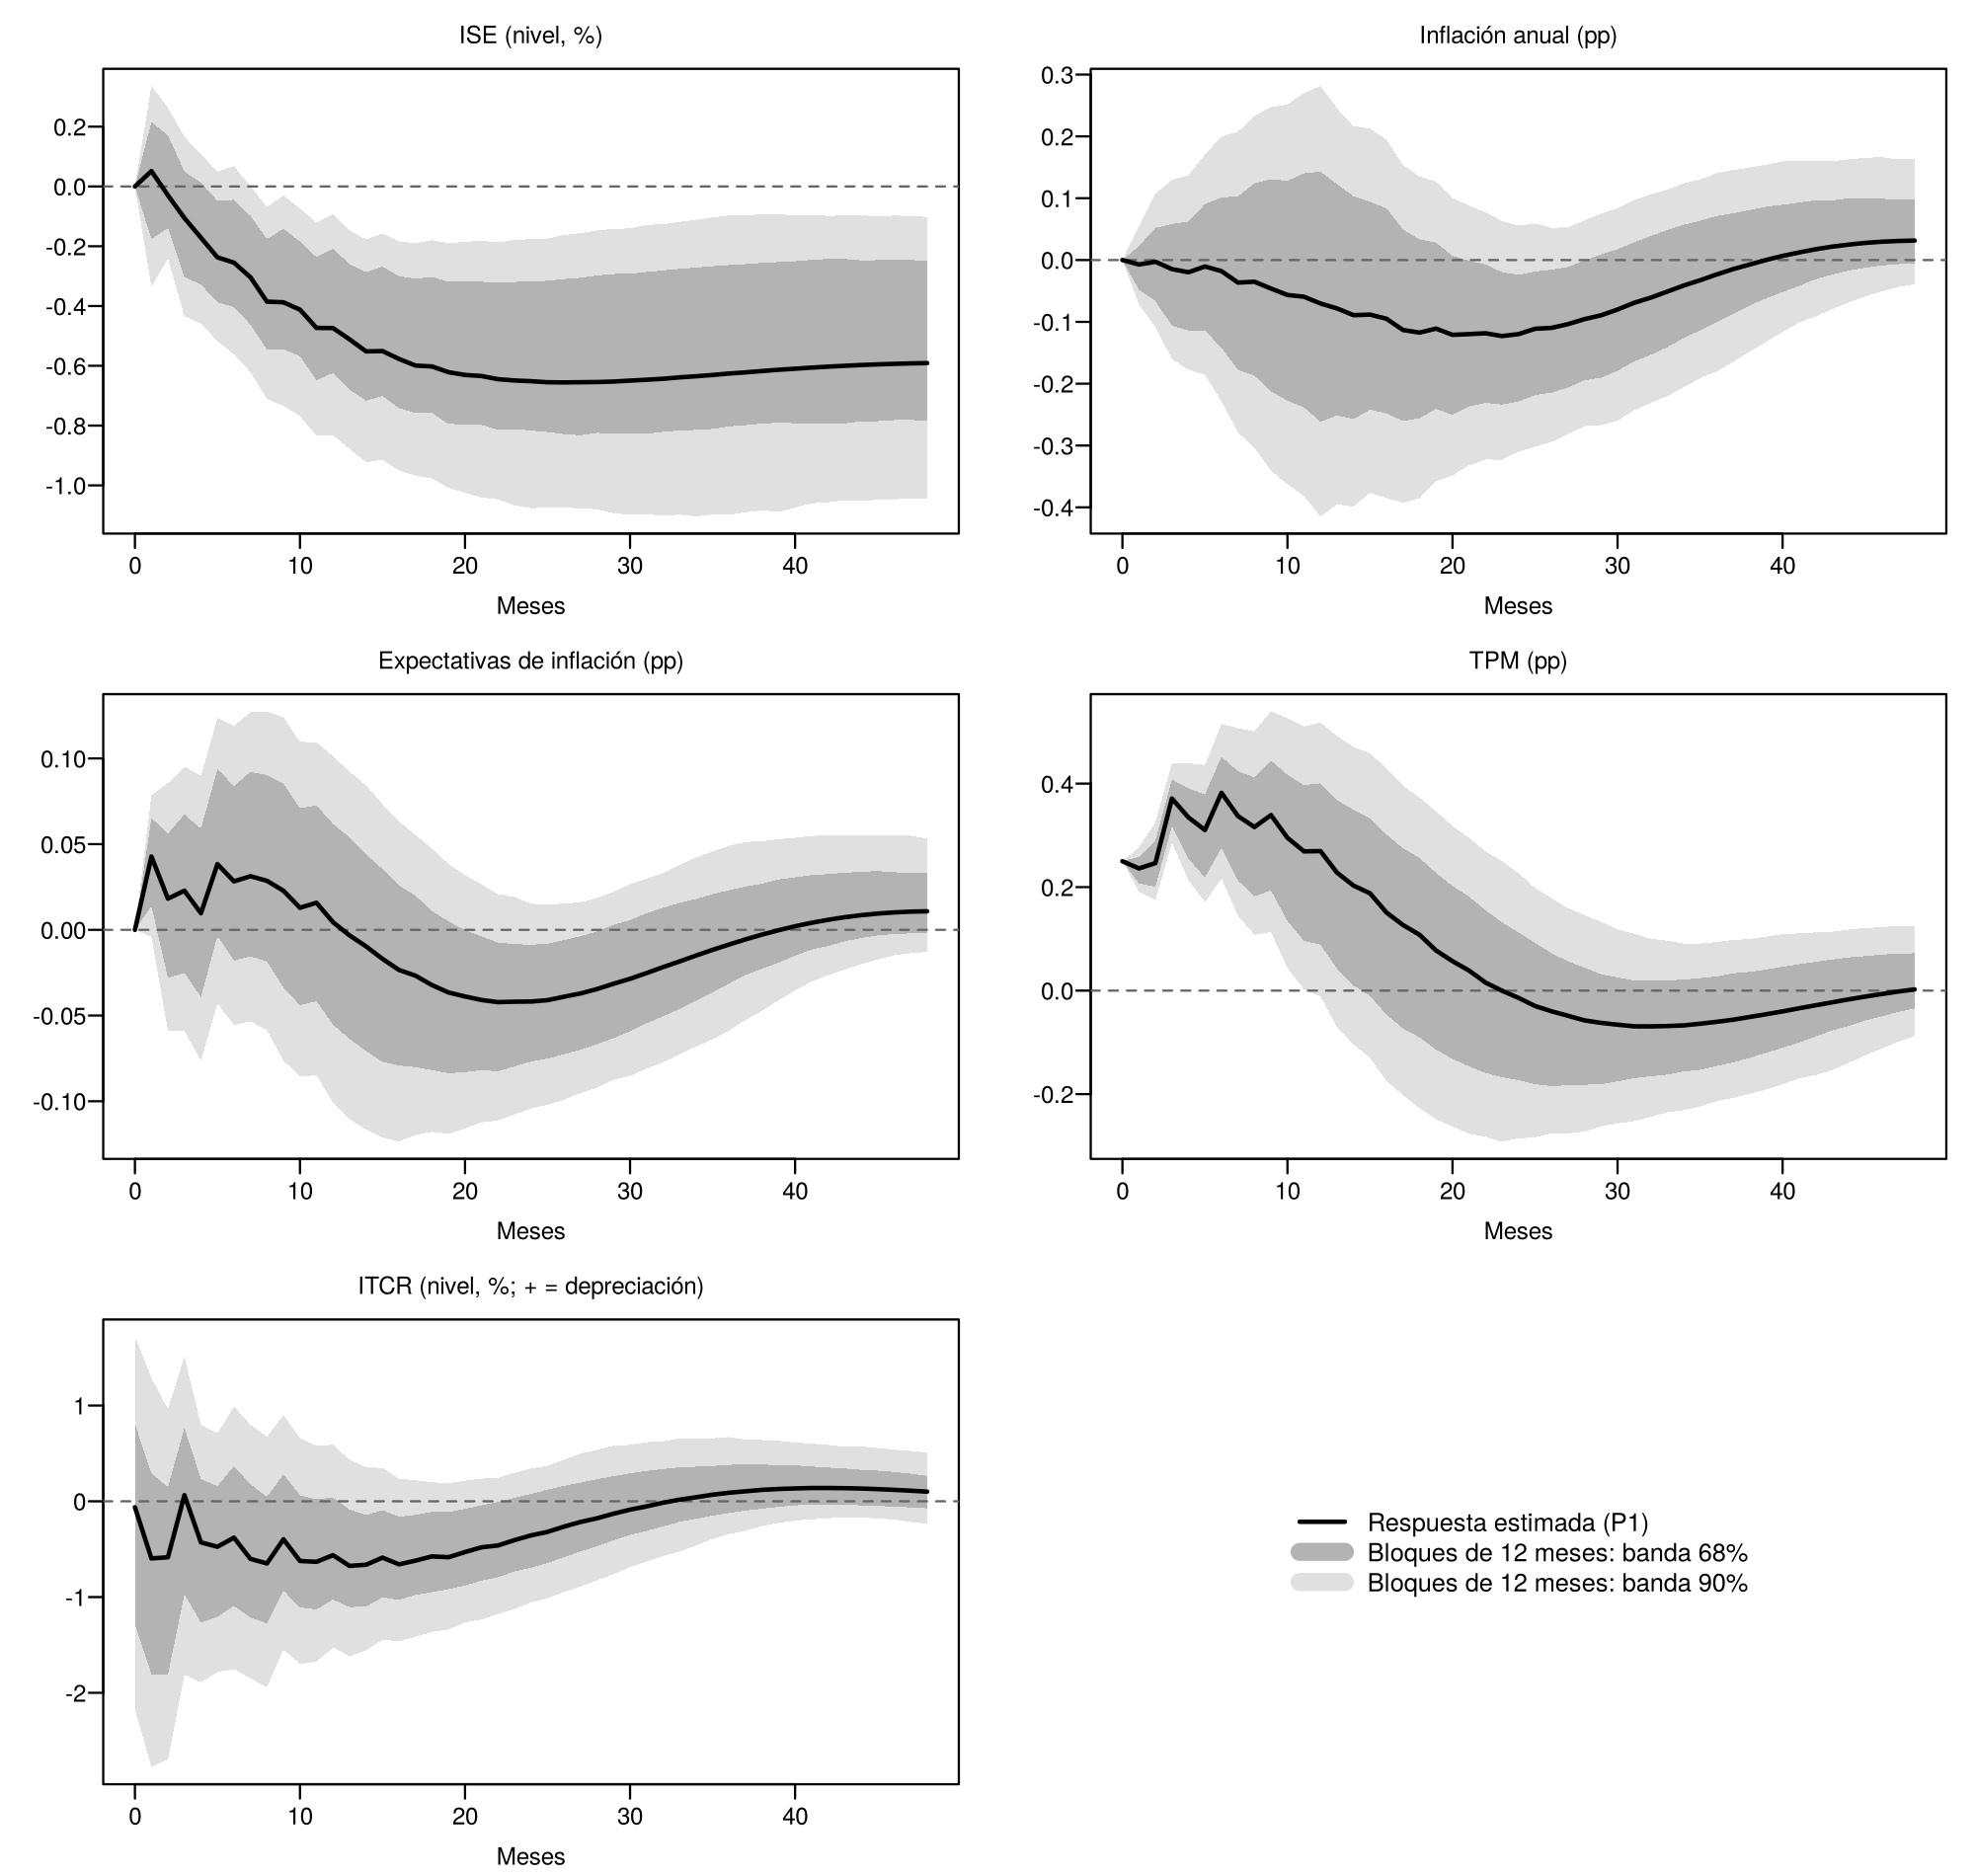
\includegraphics[height=0.68\textheight]{img/irf_P1_bloques_solo_25pb.png}
  \end{center}
  \vspace{-0.25cm}
  {\tiny \textit{Nota.} Bandas de 68\,\% y 90\,\%; 2,000 réplicas por bloques de 12 meses.\\
  Fuente: elaboración propia con datos de DANE y Banco de la República.\par}
\end{frame}

\begin{frame}{Resultados: magnitudes}
  \framesubtitle{Alza de 25 pb en la TPM: estimación y banda de 68\,\%}
  \begin{center}
  \scriptsize
  \setlength{\tabcolsep}{3pt}
  \renewcommand{\arraystretch}{1.1}
  \begin{tabular}{@{}lccccc@{}}
    \toprule
    \textbf{Variable} & \textbf{Mes 0} & \textbf{Mes 6} & \textbf{Mes 12} & \textbf{Mes 24} & \textbf{Mes 36} \\
    \midrule
    ISE & $0.00$ & $\mathbf{-0.26}$ & $\mathbf{-0.47}$ & $\mathbf{-0.65}$ & $\mathbf{-0.63}$ \\
     & --- & $[-0.40, -0.04]$ & $[-0.62, -0.21]$ & $[-0.82, -0.32]$ & $[-0.80, -0.26]$ \\
    \addlinespace
    Inflación anual & $0.00$ & $-0.02$ & $-0.07$ & $\mathbf{-0.12}$ & $-0.02$ \\
     & --- & $[-0.14, 0.10]$ & $[-0.26, 0.14]$ & $[-0.23, -0.02]$ & $[-0.10, 0.07]$ \\
    \addlinespace
    Expectativas & $0.00$ & $0.03$ & $0.00$ & $\mathbf{-0.04}$ & $-0.01$ \\
     & --- & $[-0.02, 0.08]$ & $[-0.06, 0.06]$ & $[-0.08, -0.01]$ & $[-0.03, 0.02]$ \\
    \addlinespace
    TPM & $0.25$ & $\mathbf{0.38}$ & $\mathbf{0.27}$ & $-0.01$ & $-0.06$ \\
     & --- & $[0.28, 0.45]$ & $[0.09, 0.40]$ & $[-0.17, 0.11]$ & $[-0.15, 0.03]$ \\
    \addlinespace
    ITCR & $-0.06$ & $-0.38$ & $-0.56$ & $-0.36$ & $0.09$ \\
     & $[-1.29, 0.81]$ & $[-1.09, 0.37]$ & $[-1.03, 0.04]$ & $[-0.69, 0.08]$ & $[-0.12, 0.38]$ \\
    \bottomrule
  \end{tabular}
  \end{center}
  \vfill
  {\tiny \textit{Nota.} ISE e ITCR en nivel (\%); inflación anual, expectativas y TPM en pp. Primera fila: estimación de MCO;
  segunda: percentiles 16 y 84 del bootstrap por bloques (2,000 réplicas). ---: fijado por construcción.
  En negritas: la banda de 68\,\% excluye el cero.\\
  Fuente: elaboración propia con datos de DANE y Banco de la República.\par}
\end{frame}

\begin{frame}{Robustez: rezagos}
  \framesubtitle{Respuestas a un alza de 25 pb en la TPM con 4, 6 y 8 rezagos}
  \begin{center}
    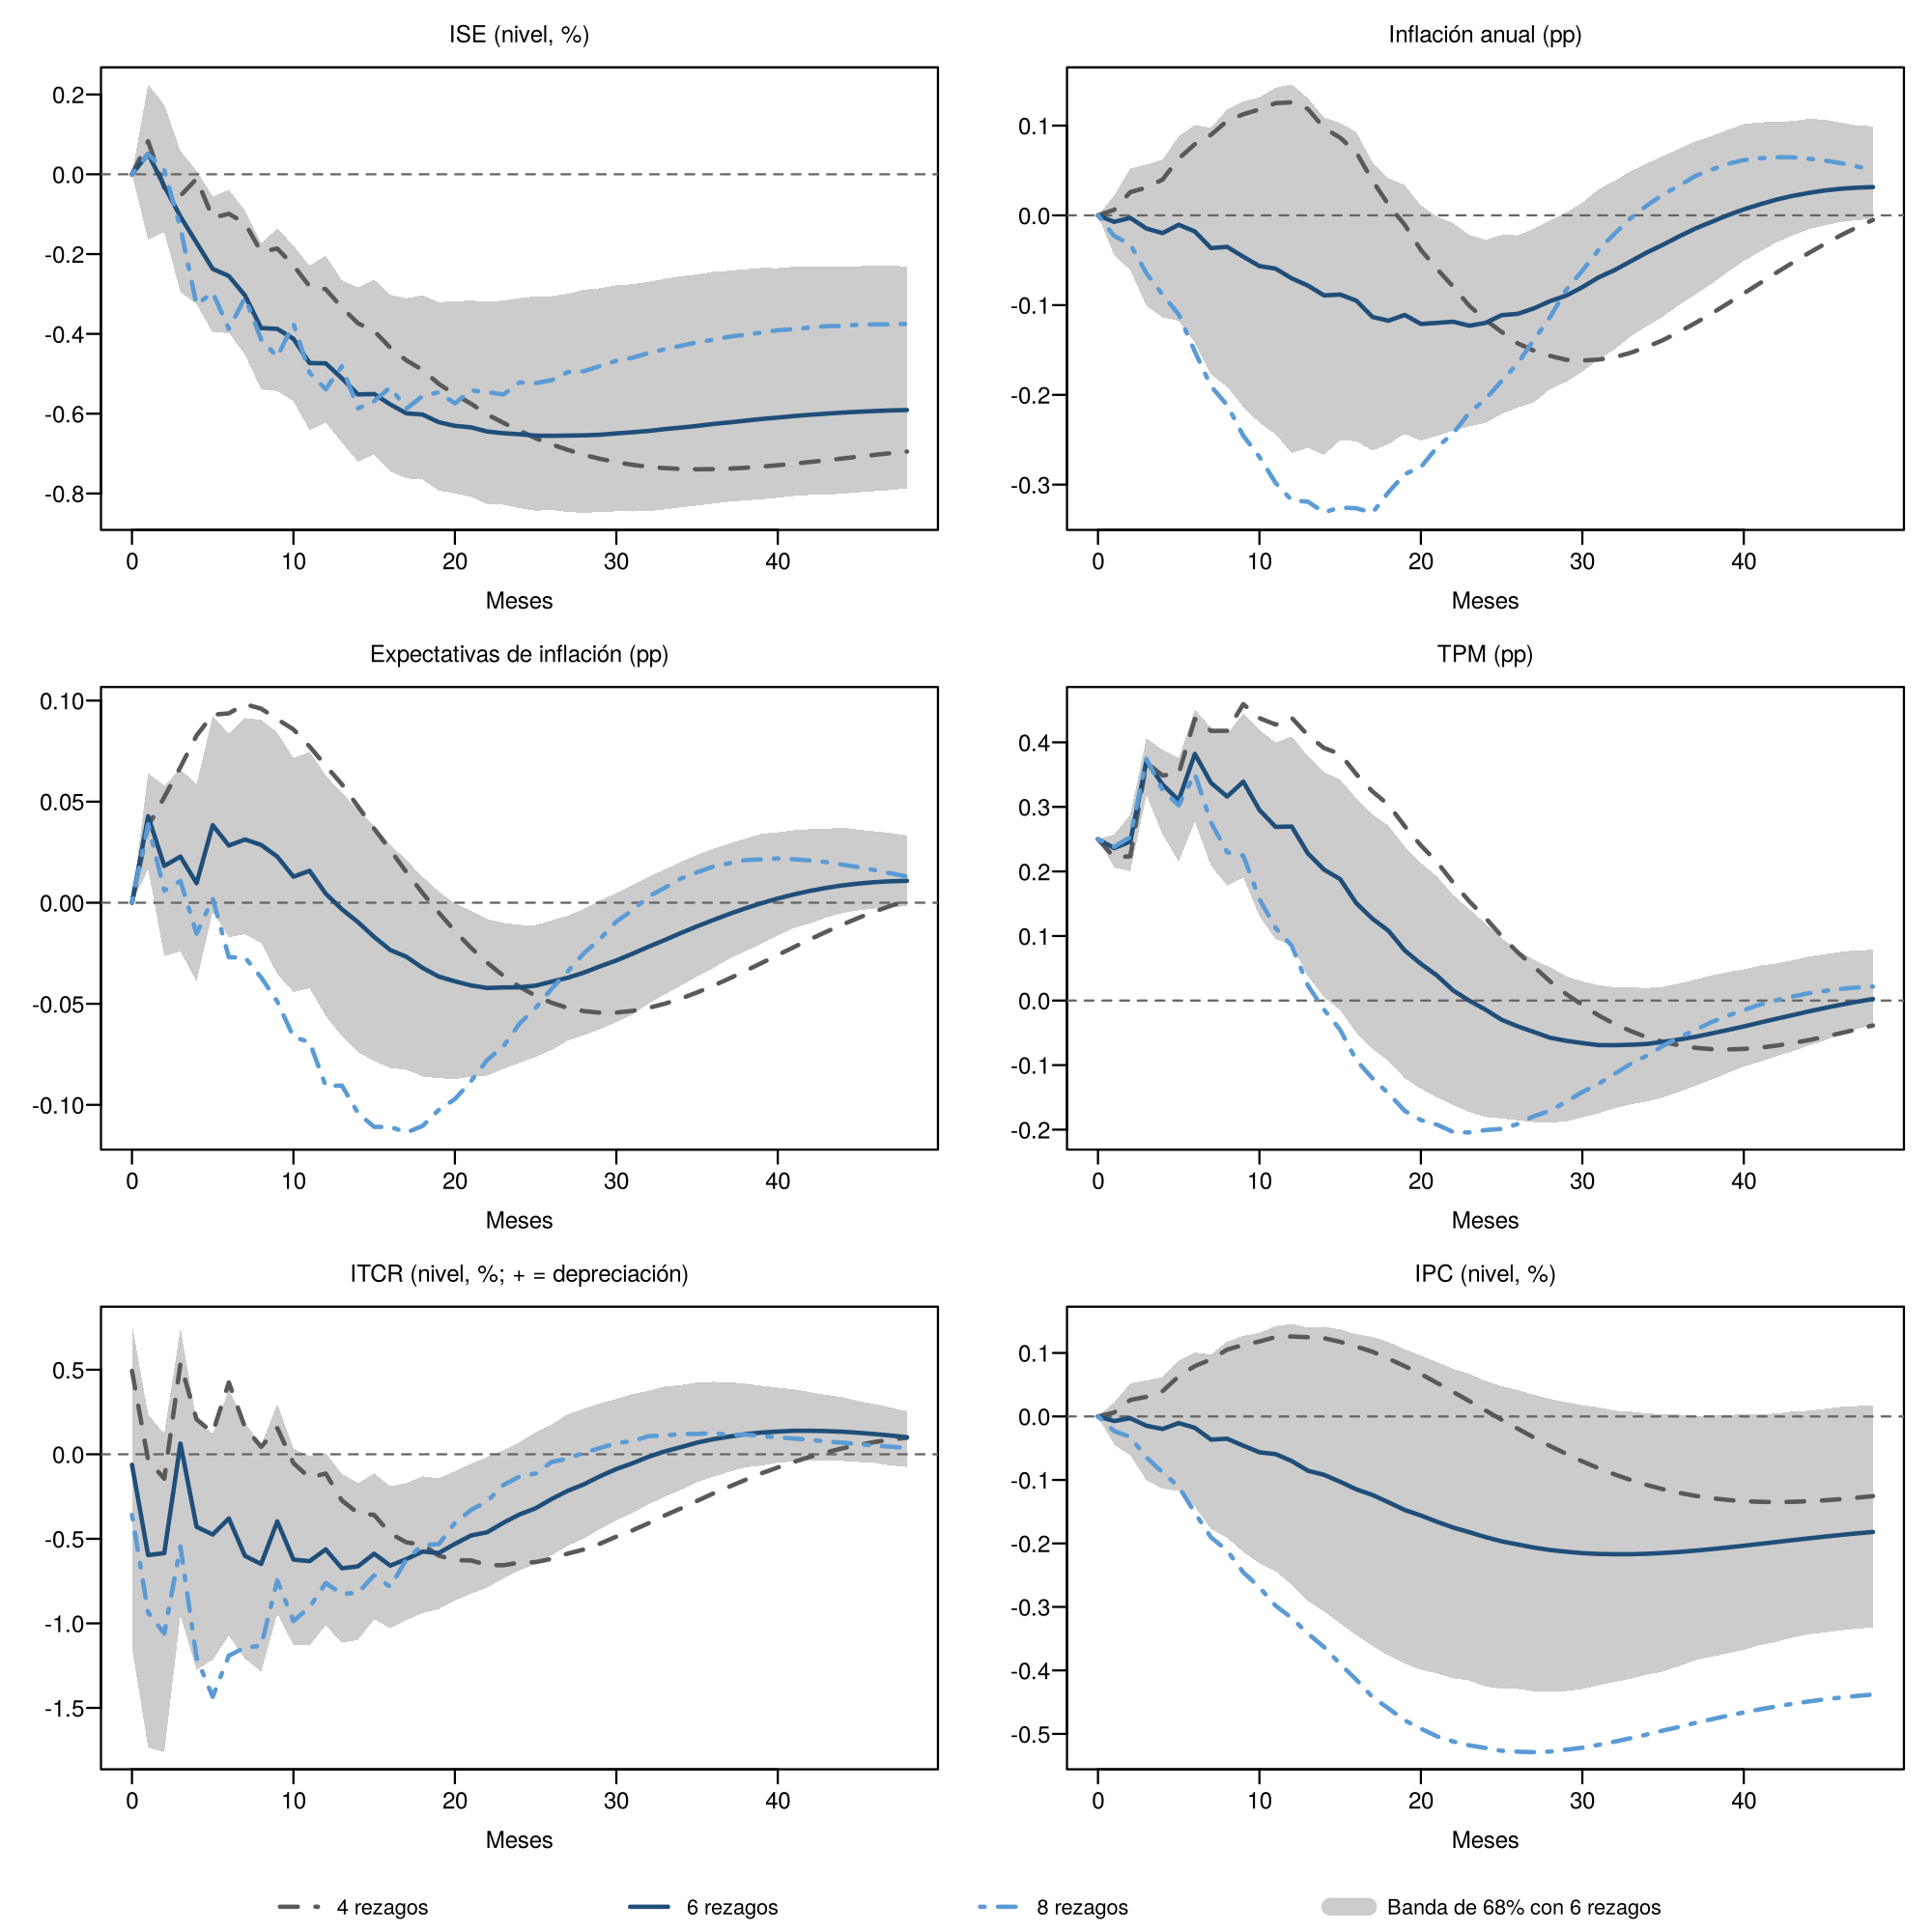
\includegraphics[height=0.68\textheight]{img/irf_P1_rezagos_25pb.png}
  \end{center}
  \vspace{-0.25cm}
  {\tiny \textit{Nota.} Banda de 68\,\% del bootstrap por bloques con 6 rezagos (2,000 réplicas).\\
  Fuente: elaboración propia con datos de DANE y Banco de la República.\par}
\end{frame}

\begin{frame}{Robustez: corrección de sesgo}
  \framesubtitle{Bandas de 68\,\%: sin corrección, con el atajo y completa}
  \begin{center}
    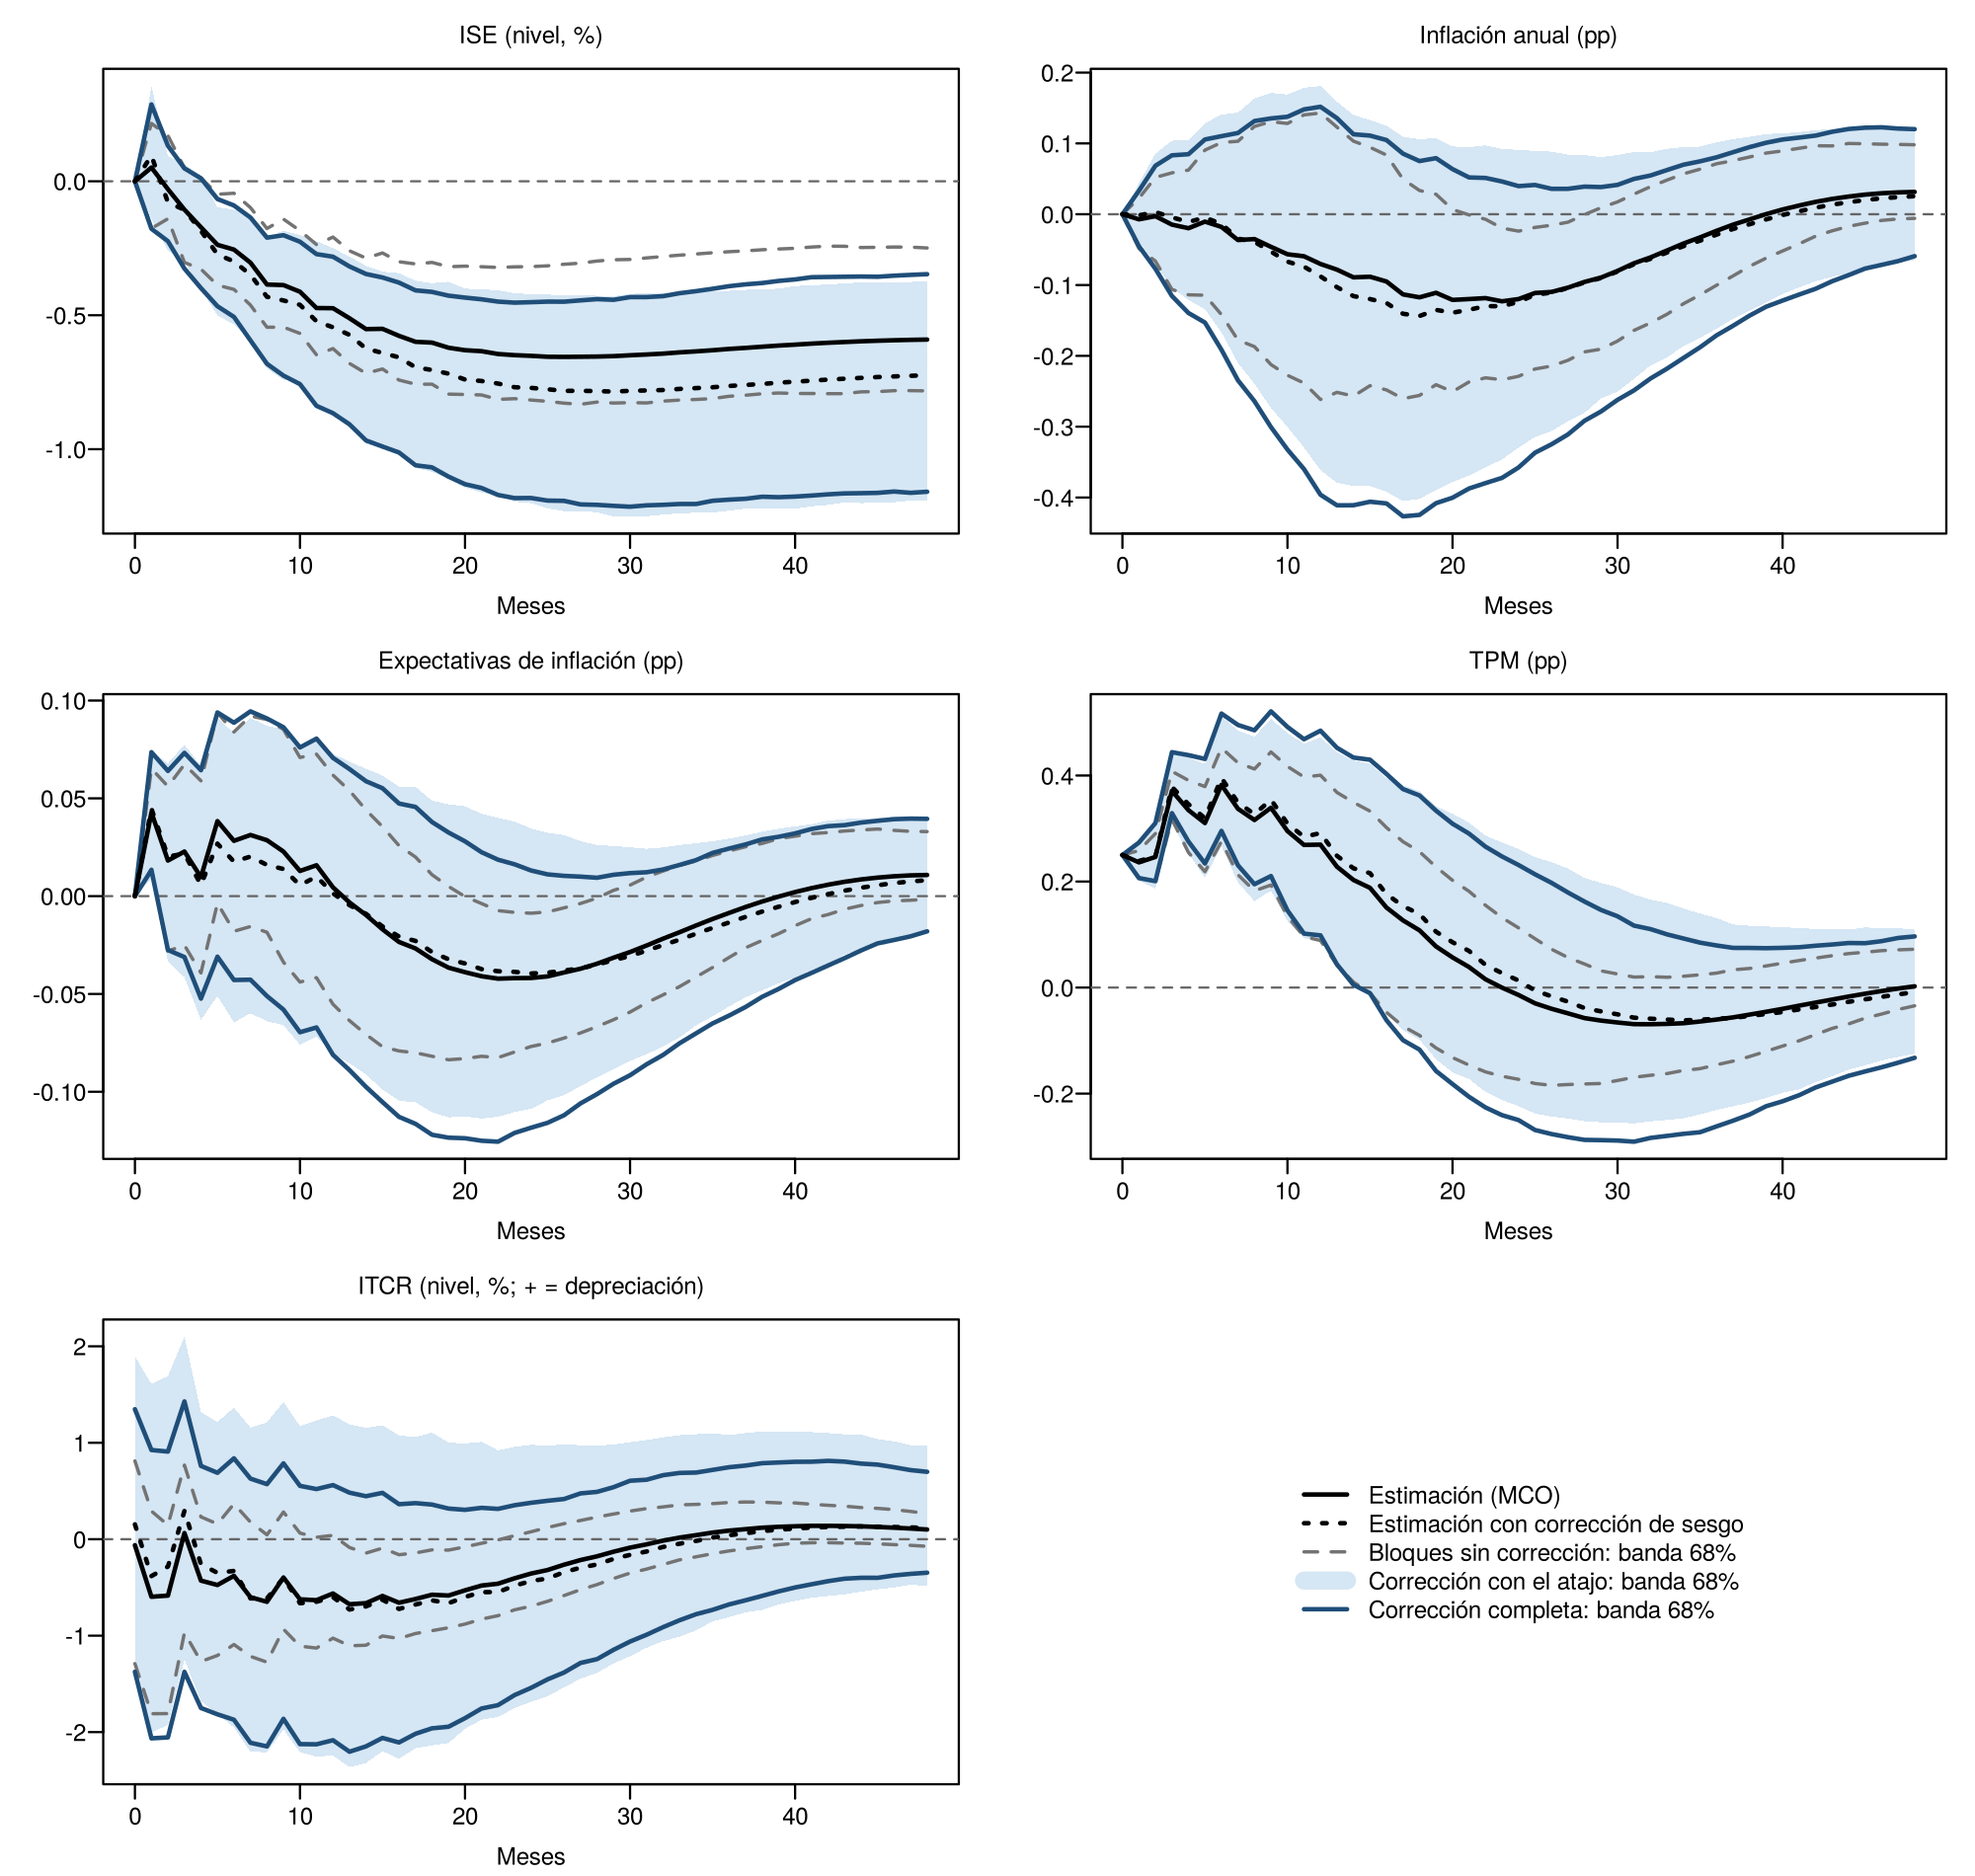
\includegraphics[height=0.68\textheight]{img/irf_P1_sesgo_completo_25pb.png}
  \end{center}
  \vspace{-0.25cm}
  {\tiny \textit{Nota.} 2,000 réplicas por bloques de 12 meses; en la corrección completa, 500 anidadas por réplica.\\
  Fuente: elaboración propia con datos de DANE y Banco de la República.\par}
\end{frame}

\begin{frame}{Robustez: distinta especificación}
  \framesubtitle{Misma forma reducida, identificación con ceros, signos y cota}
  \begin{center}
    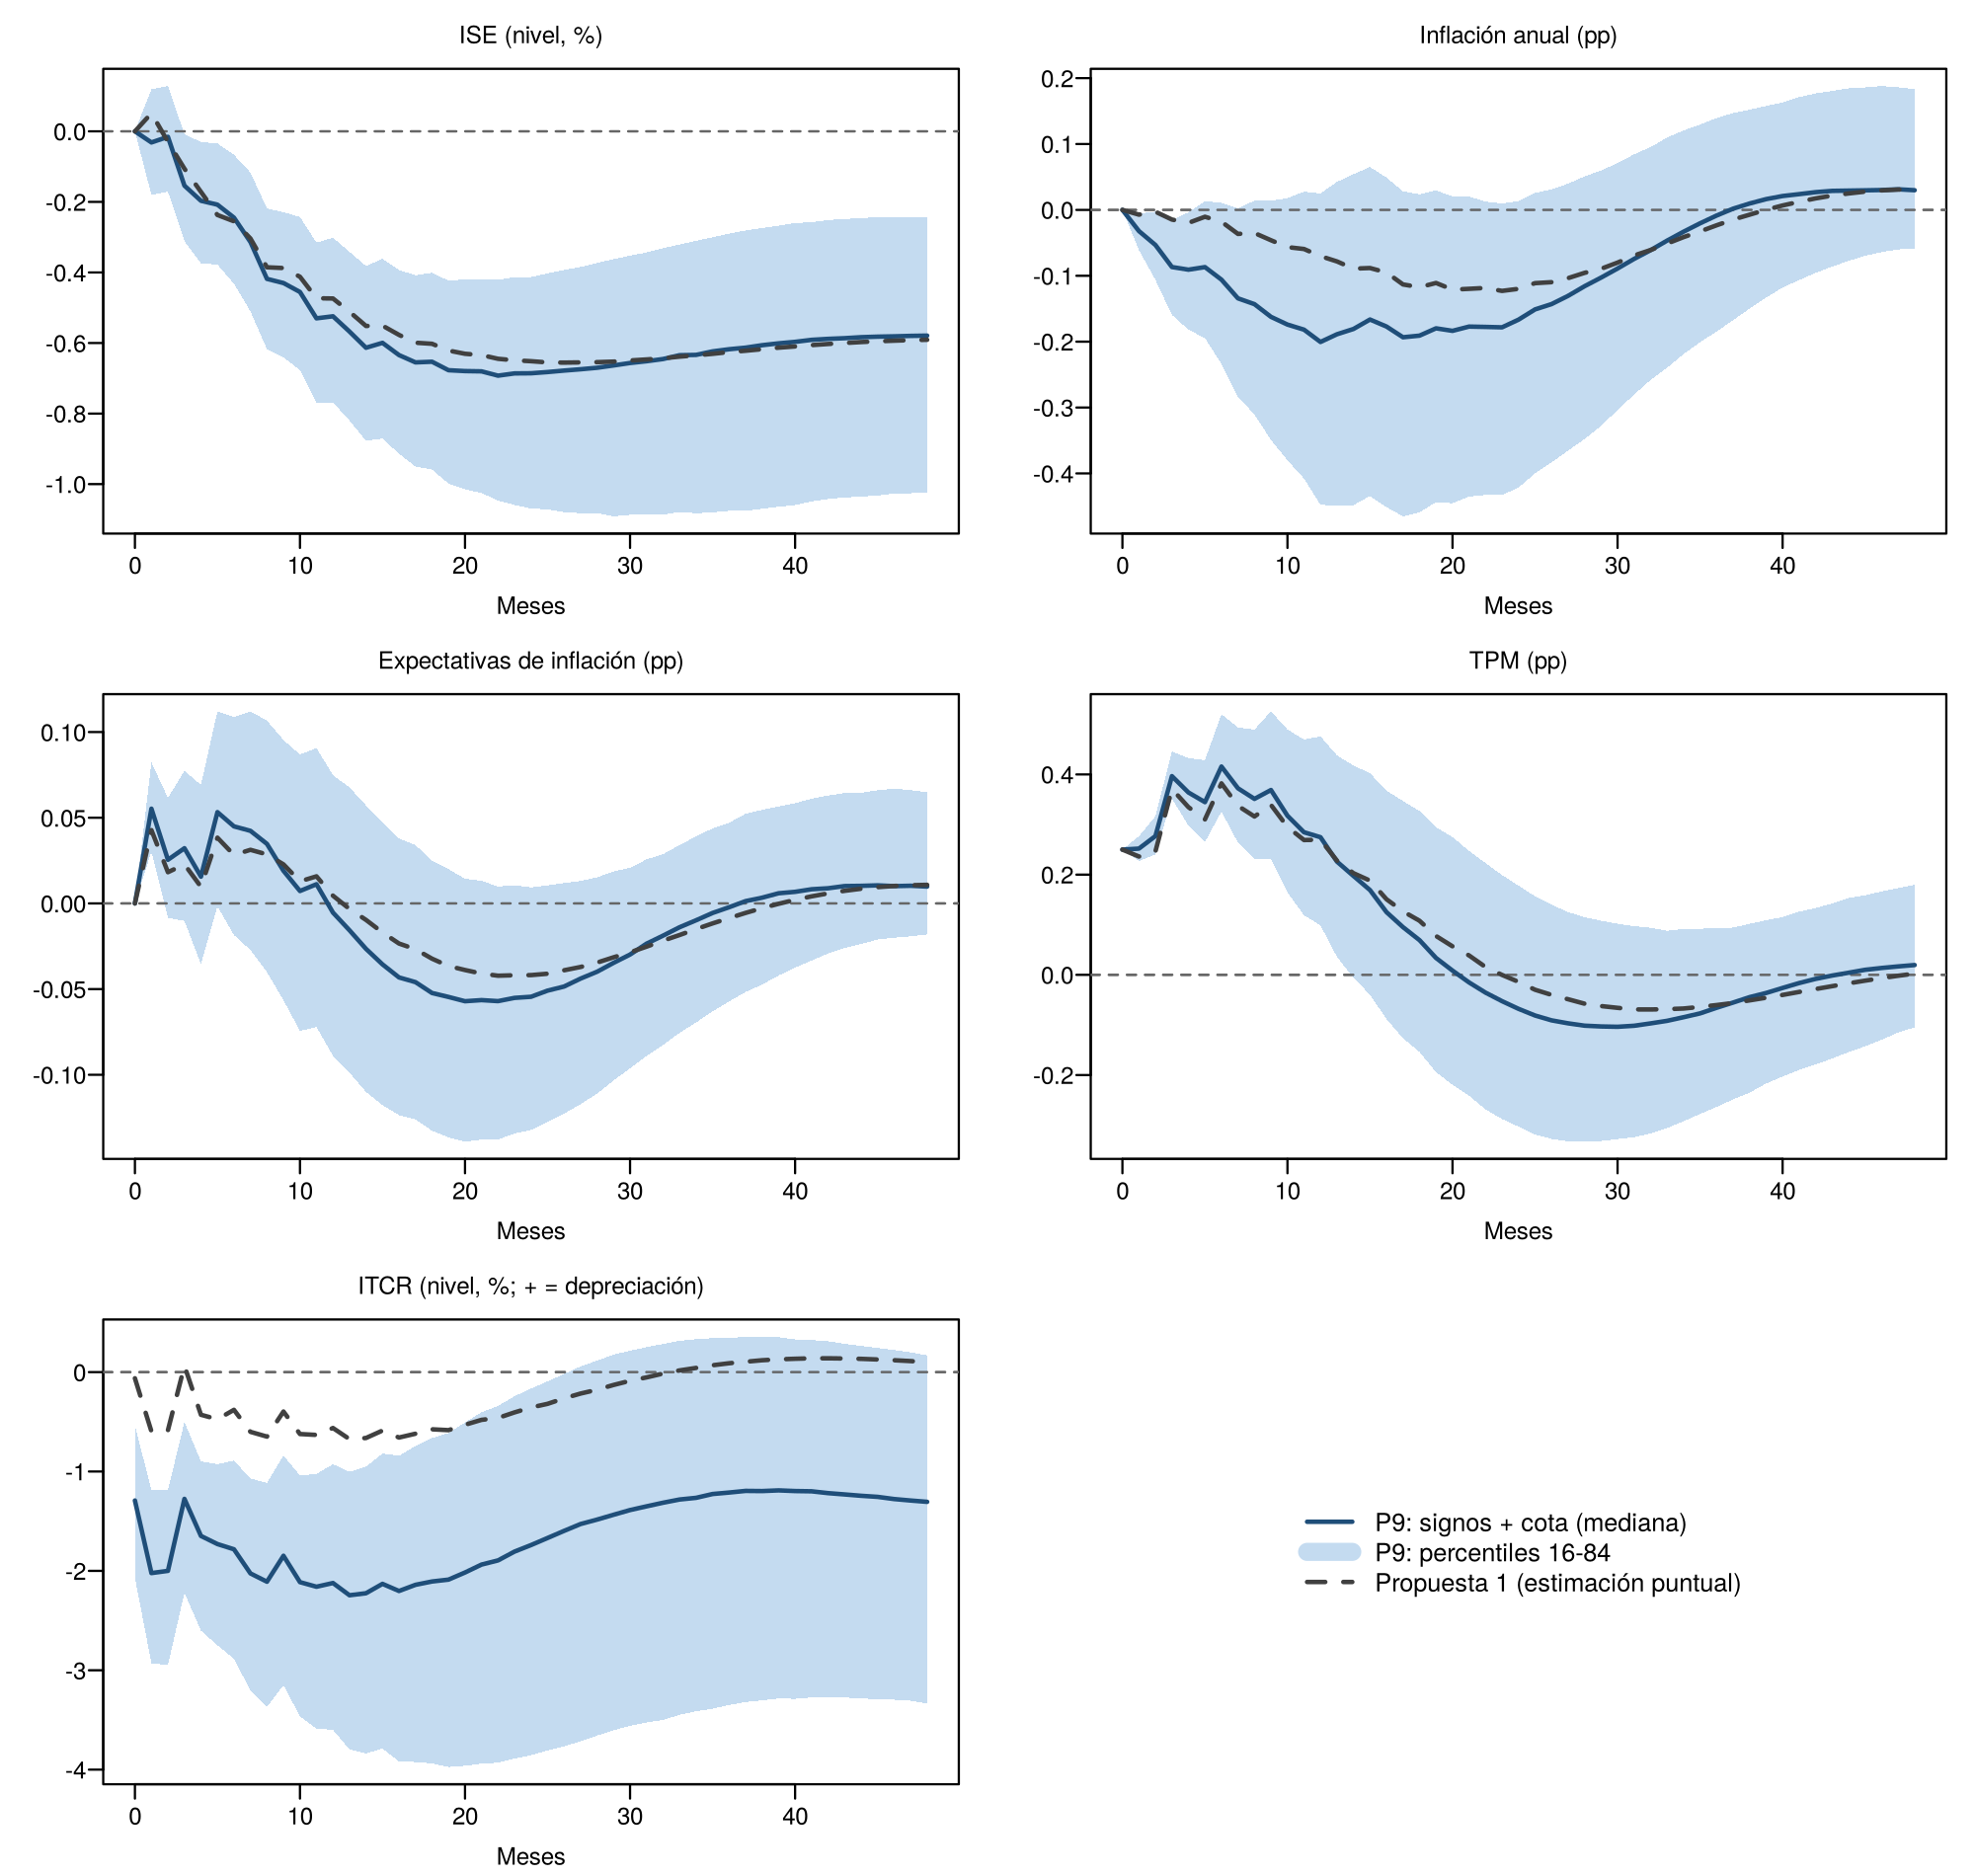
\includegraphics[height=0.68\textheight]{img/irf_P9_vs_P1_25pb.png}
  \end{center}
  \vspace{-0.25cm}
  {\tiny \textit{Nota.} Especificación 9: nueve ceros de impacto; en los meses 0 a 5 la TPM sube y el ITCR no se deprecia;
  cota $h_{54} \ge -10\,h_{44}$; 14,782 modelos aceptados. Fuente: elaboración propia con datos de DANE y BanRep.\par}
\end{frame}

% =============================================================================
\section{Conclusiones}

\begin{frame}{Conclusiones}
  \small
  \begin{enumerate}[label=(\arabic*), leftmargin=2em, itemsep=0.5em]
    \item La caída del ISE ante el alza de 25 pb en la TPM es estadísticamente significativa
    ante cualquier especificación y prueba de robustez.
    \item La inflación anual cae significativamente en distintas especificaciones, aunque no
    al corregir por sesgo.
    \item El ITCR cae con significancia estadística en diversas especificaciones, pero tampoco
    sobrevive a la corrección de sesgo.
    \item Las expectativas suben en el primer mes y luego caen hasta un mínimo en los meses
    22--23; esa caída es significativa, pero tampoco sobrevive a la corrección de sesgo.
  \end{enumerate}
  \vfill
  \begin{alertblock}{}
    \centering Sentido económico y robustez ante distintas especificaciones
    (salvo corrección de sesgo).
  \end{alertblock}
\end{frame}

\begin{frame}{Referencias}
  \scriptsize
  \setlength{\parskip}{0.45em}
  \hangindent=1.5em\hangafter=1
  Bj{\o}rnland, H. C. (2009). Monetary policy and exchange rate overshooting: Dornbusch was right after all. \textit{Journal of International Economics}, 79(1), 64--77.\par
  \hangindent=1.5em\hangafter=1
  Brüggemann, R., Jentsch, C. y Trenkler, C. (2016). Inference in VARs with conditional heteroskedasticity of unknown form. \textit{Journal of Econometrics}, 191(1), 69--85.\par
  \hangindent=1.5em\hangafter=1
  González-Téllez, C. D. y Laborde-Vera, J. C. (2026). The regional effects of monetary policy in Colombia. \textit{Borradores de Economía}, 1367. Banco de la República.\par
  \hangindent=1.5em\hangafter=1
  Kilian, L. y Lütkepohl, H. (2017). \textit{Structural Vector Autoregressive Analysis}. Cambridge University Press.\par
  \hangindent=1.5em\hangafter=1
  Larrahondo, C., Chávez, A., Giles Álvarez, L. y Andrian, L. G. (2025). The exchange rate passthrough to domestic prices: new evidence from Colombia. \textit{IDB Working Paper}, IDB-WP-01582. Banco Interamericano de Desarrollo.\par
  \hangindent=1.5em\hangafter=1
  Rowland, P. (2004). Exchange rate pass-through to domestic prices: the case of Colombia. \textit{Ensayos sobre Política Económica}, 22(47), 106--125.\par
  \hangindent=1.5em\hangafter=1
  Sánchez-Jabba, A. y Villabón-Hinestroza, E. (2024). The measure matters: differences in the passthrough of inflation expectations in Colombia. \textit{BIS Working Papers}, 1205. Bank for International Settlements.\par
\end{frame}

\begin{frame}[plain,noframenumbering]
  \vfill
  \begin{center}
    {\fontsize{30}{34}\selectfont\bfseries\color{azulraf}¡Gracias!\par}
    \vspace{0.35cm}
    {\color{azulraf}\rule{0.35\textwidth}{1.2pt}\par}
    \vspace{0.5cm}
    {\small Oscar Daniel Hernández Romero \textperiodcentered\ Kevin Mejía Rodríguez \textperiodcentered\ Rubén Perea Cervantes\par}
  \end{center}
  \vfill
\end{frame}


\end{document}
